\documentclass[12pt, letterpaper]{article}
\usepackage[utf8]{inputenc}
\usepackage{amsmath,amsfonts,amssymb, mathtools, geometry, algorithm, algorithmic, graphicx, wrapfig, float, hyperref, array, xurl,setspace,tocloft, tikz, titlesec, caption,amsthm,enumitem,bm}
\makeatletter
\renewcommand*\env@matrix[1][\arraystretch]{%
  \edef\arraystretch{#1}%
  \hskip -\arraycolsep
  \let\@ifnextchar\new@ifnextchar
  \array{*\c@MaxMatrixCols c}}
\makeatother

\geometry{margin=1in}
\doublespacing
\graphicspath{{images/}}

\titlespacing\section{0pt}{0pt}{0pt plus 2pt minus 2pt}
\titlespacing\subsection{0pt}{5}{0pt plus 2pt minus 2pt}
\titlespacing\subsubsection{0pt}{5}{0pt plus 2pt minus 2pt}
\captionsetup{belowskip=-15pt}


\title{Visualising 4D Polygons}
\author{}
\date{}
\begin{document}
\setlength{\abovedisplayskip}{5pt}
\setlength{\belowdisplayskip}{5pt}
\allowdisplaybreaks
\begin{tikzpicture}[overlay, remember picture]
\path (current page.north east) ++(-1,-1) node[below left] {};
\end{tikzpicture}
\vspace{-0.9cm}
\begin{center}
    Mathematics IA\\
    \vspace{-0.5cm}
    \huge
    \textbf{Visualizing 4D Polygons}\\
    \normalsize
    \vspace{0.2cm}
    \normalsize
    How can 4D shapes be visualized by humans?
    \vspace{-0.4cm}\\
\end{center}

\section{Introduction and Rationale}
4D is an elusive concept popularized in many aspects of human media and culture; movies, books, and people all seem to talk about 4D in some way. But what are 4D shapes, and how can humans perceive them? 

As a computer graphics enthusiast, I have made many different types of physics simulations. All of which have been constrained to 3D space and lower. As I moved from 2D to 3D, the complexity of geometric interactions increased, and I observed interesting phenomena regarding the change in spatial volume. These observations raised an important question: what happens if I go beyond 3D space? To satisfy my curiosity, I investigated how the visualization of 4D shapes work. Moreover, creating a complete rendering engine is also a long-term goal of mine. I am also deeply intrigued by the ability of mathematical abstraction to help visualize concepts beyond human perception. Therefore, as an investigation of 4D visualization, the goal of this IA is to find a transformation matrix that can project any 4D wireframe into human-perceivable 3D space. (Note: all diagrams in this IA are self-created by the author)

\section{Human Perception and Perspective Projections}
 To visualize 4D, it is meaningful to discuss how humans perceive objects in general. In reality, humans actually cannot see 3D space directly. Instead, humans only see a 2D projection of light onto their retinas. The sense of 3D in human sight is an illusion caused by shadows, lights, parallax with two eyes, and clever brain trickery. Fundamentally, the eye can be simplified into a few key components: the lens, the focal point, and the retina. The retina is the 2D plane to which the light will be projected, and the focal point is the pivot that gives the 3D object perspective.
\begin{figure}[H]
\centering
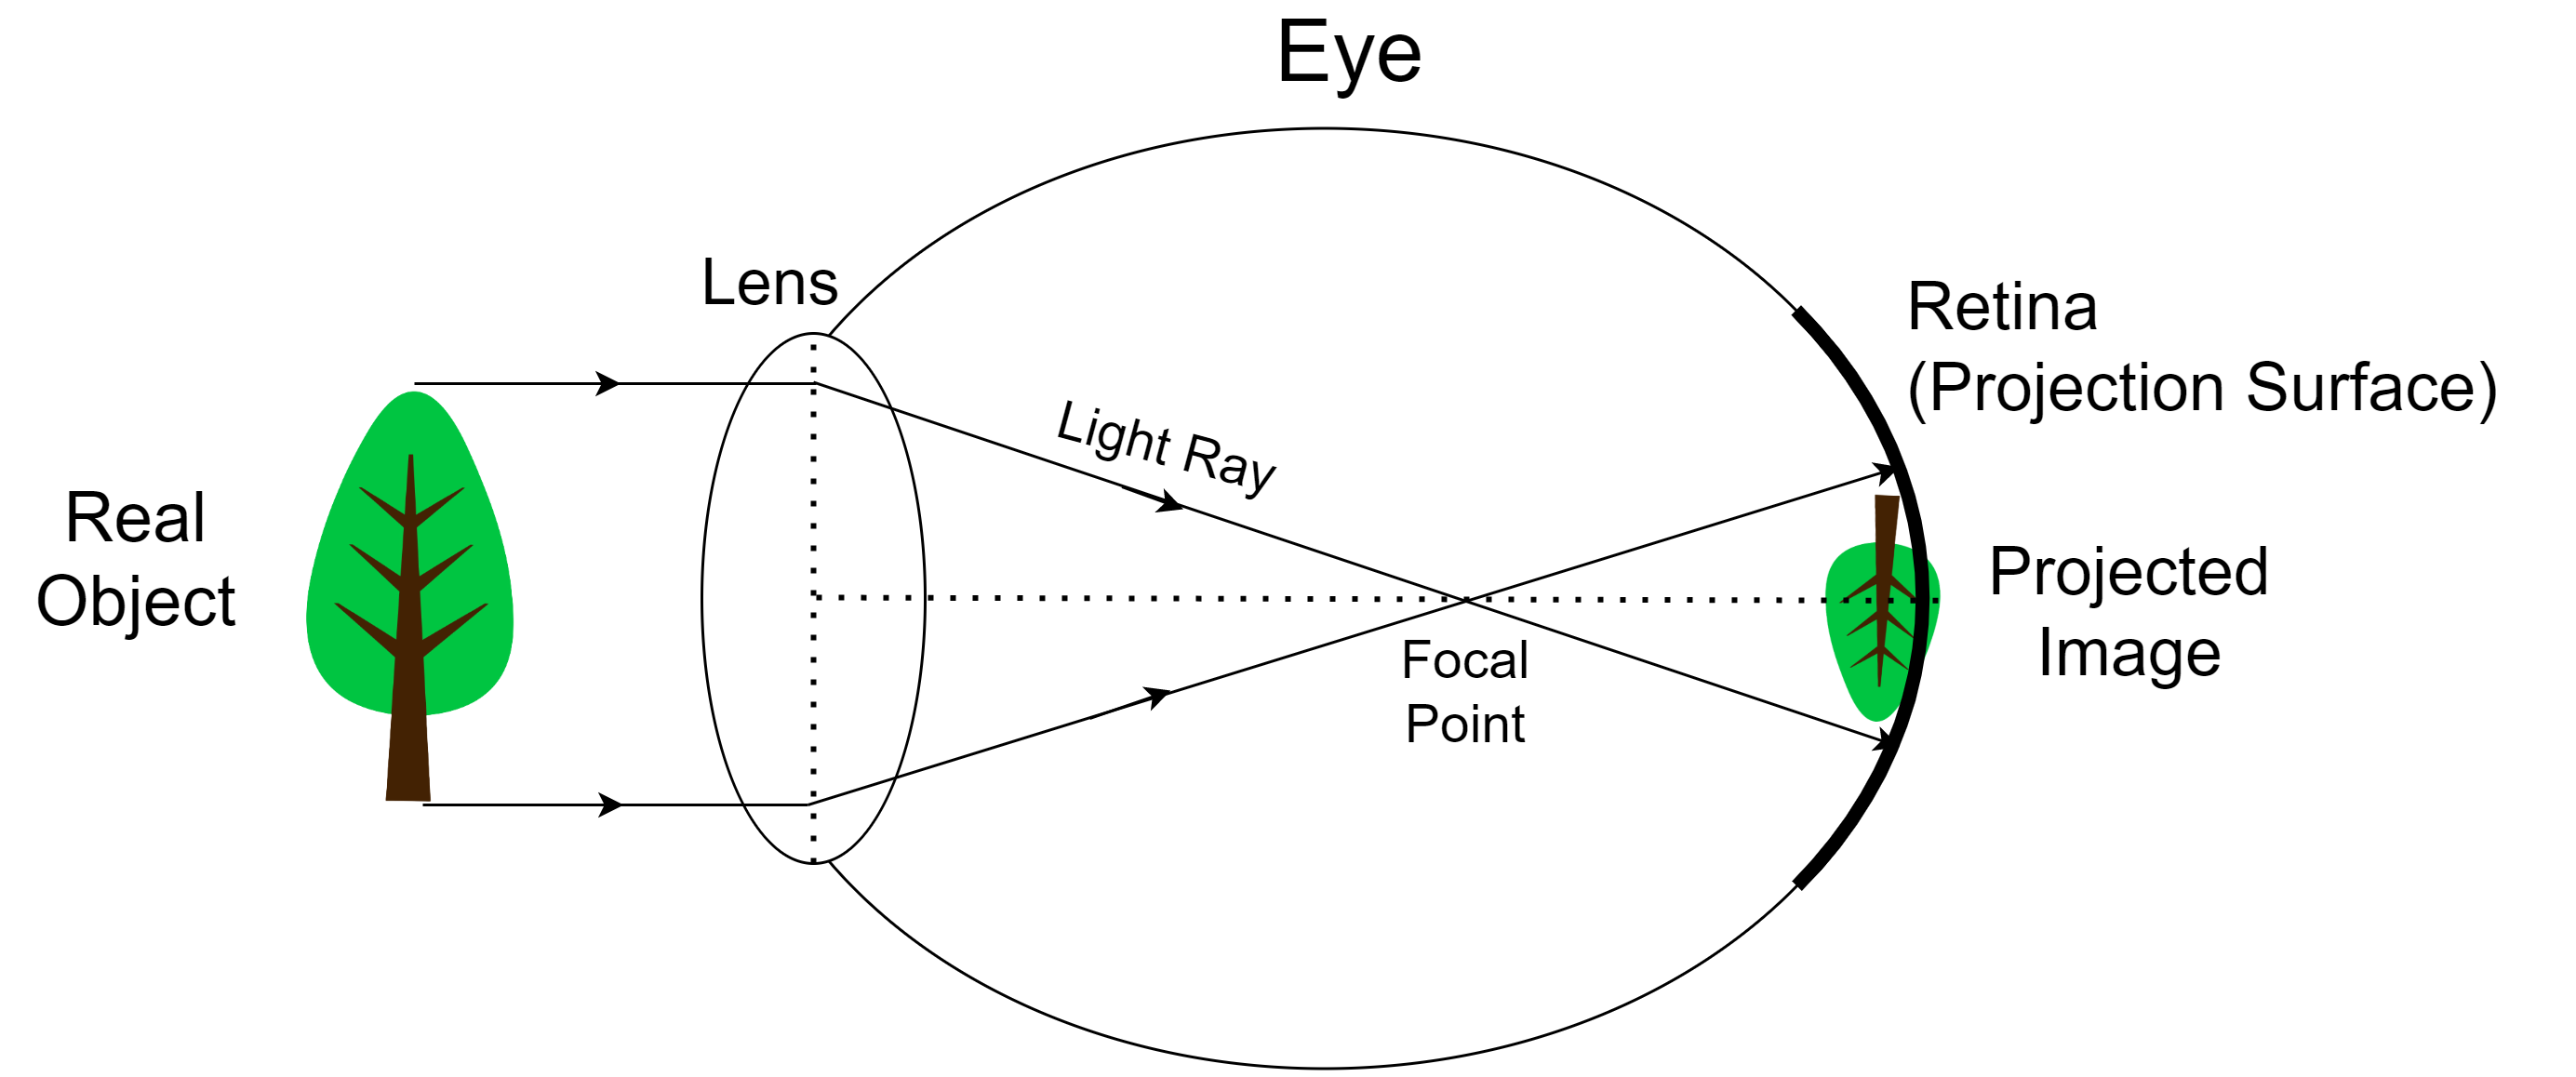
\includegraphics[width=12cm]{eye.png}
\caption{Diagram of the human eye}
\label{fig:figure}
\end{figure} 
For this IA, the projection will use the same principles as the eye diagram, with the exception that the retina at the end is flat (Figure 2). The approach taken is closer to that of a pinhole camera.
\begin{figure}[H]
\centering
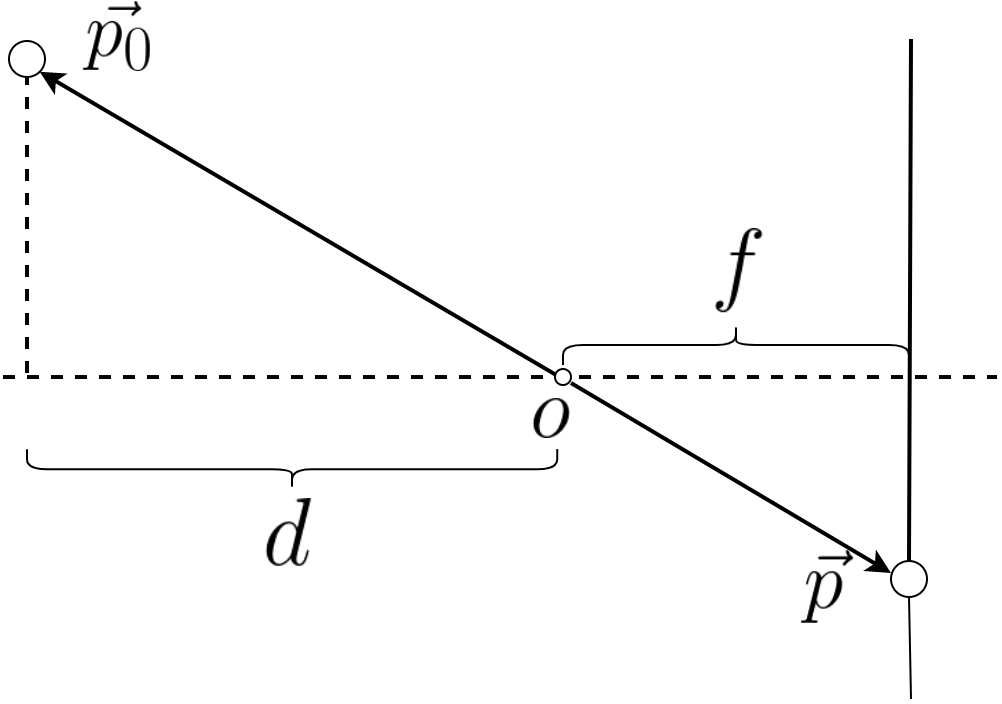
\includegraphics[width=7cm]{simple_eye.png}
\caption{Diagram of the simplified projection system of the eye. }
\label{fig:figure}
\end{figure} 
In the diagram, $\vec{p_0}$ is the position vector of the original point, $\vec{p}$ is the position vector of the projected point, and $o$ is the origin. The scalars $d$ and $f$ represent the distance to the focal point and the focal distance respectively. However, the projected object is inverted, and inversion is not ideal because it is not the ``real" orientation of the original object. To simplify the projection process, the ``retina" (the 2D plane) will be moved to the front of the focal point instead. This still results in a perspective projection because the projection is still scaled by the distance between the original object and the focal point. 
\begin{figure}[H]
\centering
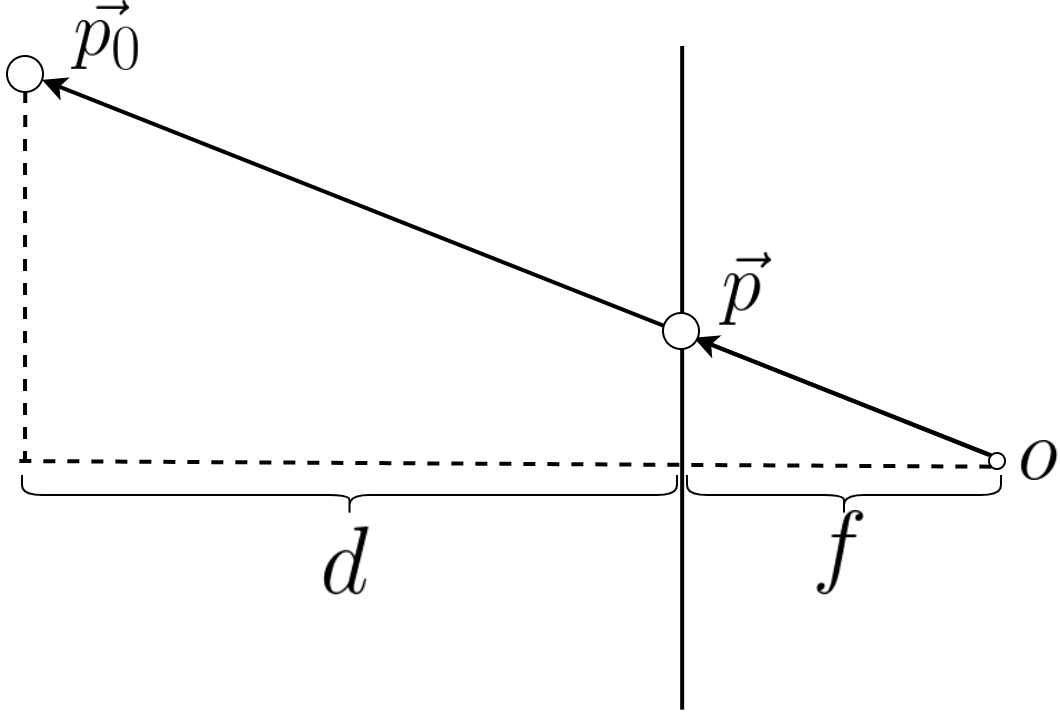
\includegraphics[width=6cm]{edited_eye.png}
\caption{Diagram of the projection system used for this IA}
\label{fig:figure}
\end{figure} 
This will form the basis of perspective projections, and the next sections will formalize this result with mathematics.

\section{Definitions and Notation}
The 4th dimensional axis will be denoted as $w$. Components of a vector $\vec{v_1}$, will be referred as $v_{1,n}$. To illustrate, the x-component of $\vec{v_1}$ will be $v_{1,x}$. Matrices will be represented as capitalized letters with a bold font, ie, $\mathbf{A}$. The vectors for this IA will be slightly different from typical spacial vectors. First of all, vectors will be in row form. Meaning, 
$\vec{v} = x\vec{i} + y\vec{j} + z\vec{k} = \begin{bmatrix}[0.5]x&y&z\end{bmatrix}$. Hence, the vector basis will also be in row form, where for 3D $\vec{i} = \begin{bmatrix}[0.5]1&0&0\end{bmatrix}$, $\vec{j} = \begin{bmatrix}[0.5]0&1&0\end{bmatrix}$, $\vec{k} = \begin{bmatrix}[0.5]0&0&1\end{bmatrix}$. Similarly, the vector basis in 4D will be represented as $\vec{i} = \begin{bmatrix}[0.5]1&0&0&0\end{bmatrix}$, $\vec{j} = \begin{bmatrix}[0.5]0&1&0&0\end{bmatrix}$, $\vec{k} = \begin{bmatrix}[0.5]0&0&1&0\end{bmatrix}$, and $\vec{l} = \begin{bmatrix}[0.5]0&0&0&1\end{bmatrix}$. This form was specifically chosen because it is easier to implement programmatically. Because of this, the order of vector and matrix multiplication will be reversed. In other words, multiplication will be in the order of $\vec{v} \mathbf{A}$. Moreover, an additional dimension will be added to all vectors. Therefore, a 3D vector will be represented as $\begin{bmatrix}[0.5]x&y&z&1\end{bmatrix}$, and 4D as $\begin{bmatrix}[0.5]x&y&z&w&1\end{bmatrix}$. The additional 1 at the end of each vector will enable translation matrices, $\mathbf{D}$, where $\vec{v}\mathbf{D} = \vec{v'}$. Vectors written in this form have homogeneous coordinates, and any transformations on homogeneous coordinates are called affine transformations (Strang). As a result, 3D spacial vectors will have 4 components, and 3D transformation matrices will be $4 \times 4$. Similarly, 4D spacial vectors will have 5 components, and 4D transformation matrices will be $5 \times 5$.

\section{3D Perspective Projections}
 Because it is not possible for a human to directly visualize 4D space, a projection process is first developed for 3D space and later extended to 4D. Having an understanding of 3D perspective projections to a 2D space will allow the development of some key aspects of the entire process. This section will discuss how to project 3D points onto 2D space, as points (vertices) are a key component of polygons.
\begin{figure}[H]
\centering
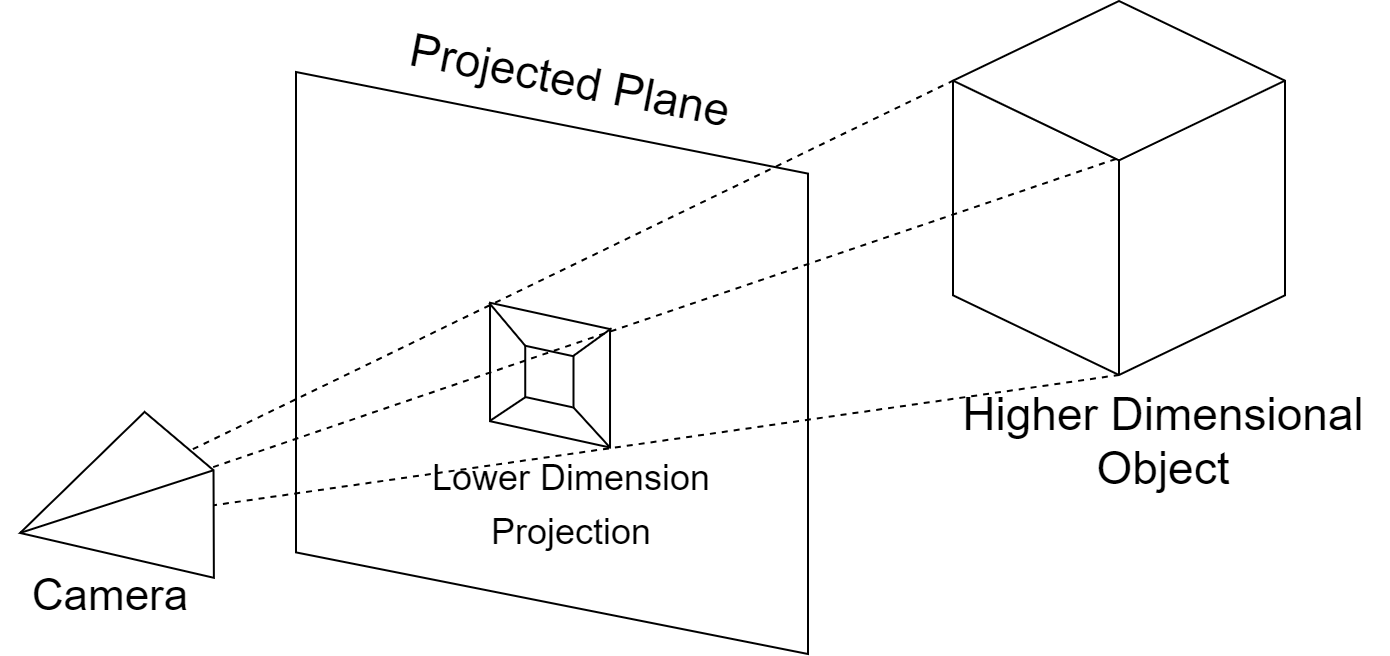
\includegraphics[width=8.5cm]{3d_projection_diagram.png}
\caption{The general 3D projection process}
\label{fig:figure}
\end{figure} 
\subsection{Simple Perspective Projection Case}
This section will be guided by the following diagram
\begin{figure}[H]
\centering
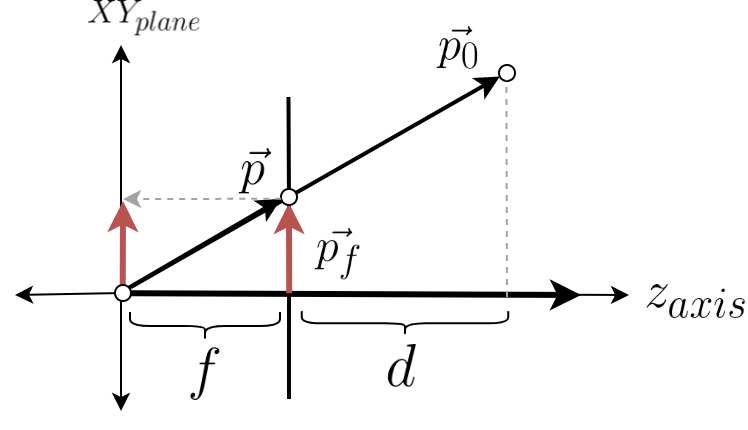
\includegraphics[width=8.5cm]{simple_3D.png}
\caption{Simple 3D projection}
\label{fig:figure}
\end{figure} 
The key to perspective projections is to find the value of $\vec{p_f} \in \mathbb{R}^4$, given $\vec{p_0}\in \mathbb{R}^4$, $f \in \mathbb{R}_{\geq0}$, and $d \in \mathbb{R}_{\geq0}$. The final projection $\vec{p_f}$ is in the 2D plane of which it is projected to. This IA also assumes that the projected plane extends infinitely. To solve for this value, $\vec{p}$ is first calculated using similar triangles. Because the triangle of $\vec{p_0}$ shares two angles as the triangle of $\vec{p}$, they are similar triangles. Therefore by comparing sides, 
$$\frac{|\vec{p_0}|}{f+d} = \frac{|\vec{p}|}{f}.$$
Hence, isolating $\vec{p}$ yields
$$|\vec{p}| = \frac{f}{f+d}|\vec{p_0}|.$$
Because $\vec{p}$ and $\vec{p_0}$ are collinear, $\vec{p}$ must be a scalar multiple of $\vec{p_0}$, and the scalar value must also be same as the scaling for the length. Furthermore, the value $f+d$ is simply just the z-coordinate of the point $\vec{p_0}$. Which results in,
\begin{equation}
    \vec{p} = \frac{f}{p_{0, z}}\vec{p_0}.
\end{equation}
This scaling on $\vec{p_0}$ can be rewritten as a scaling matrix, $\mathbf{S}$, that applies the scalar multiple to each component of $\vec{p_0}$. Hence, 
$$\vec{p} = \vec{p_0} \begin{bmatrix}[0.7] \frac{f}{p_{0,z}} & 0 & 0 & 0\\ 0 & \frac{f}{p_{0, z}} & 0 & 0 \\ 0 & 0 & \frac{f}{p_{0, z}} & 0 \\ 0 & 0 & 0 & 1\\   \end{bmatrix}.$$
Next, to get the position vector $\vec{p_f}$ in the plane of projection (the 2D plane), $\vec{p}$ needs to be translated along the z-axis. The translation will displace the same length as the focal distance, $f$, and because it is along the z-axis, only the z-component will be affected. To keep everything consistent, a $4\times4$ translation matrix will be used. The result then is
$$\vec{p_f} = \vec{p} \begin{bmatrix}[0.6] 1 & 0 & 0 & 0\\ 0 & 1 & 0 & 0 \\ 0 & 0 & 1 & 0 \\ 0 & 0 & -f & 1\\   \end{bmatrix}.$$
Translation matrices is the reason why homogeneous coordinates were used, since expanding this translation gives $\vec{p_f} = \begin{bmatrix}[0.5]p_{x}&p_{y}&(p_{z}-f)&1 \end{bmatrix}$. The last step combines the translation and projection results in the final projection matrix, $\mathbf{J}$. Where, 
\begin{equation}
    \mathbf{J} = \begin{bmatrix}[0.6] \frac{f}{p_{0, z}} & 0 & 0 & 0\\ 0 & \frac{f}{p_{0, z}} & 0 & 0 \\ 0 & 0 & \frac{f}{p_{0, z}} & 0 \\ 0 & 0 & 0 & 1\\   \end{bmatrix} \begin{bmatrix}[0.6] 1 & 0 & 0 & 0\\ 0 & 1 & 0 & 0 \\ 0 & 0 & 1 & 0 \\ 0 & 0 & -f & 1\\   \end{bmatrix} = \begin{bmatrix}[0.7] \frac{f}{p_{0, z}} & 0 & 0 & 0\\ 0 & \frac{f}{p_{0, z}} & 0 & 0 \\ 0 & 0 & \frac{f}{p_{0, z}} & 0 \\ 0 & 0 & -f & 1\\   \end{bmatrix}
\end{equation}
and $\vec{p_f} = \vec{p_0}\mathbf{J}$.

\subsection{Translated Camera Coordinates}
The camera coordinates do not always need to be at the origin, and they could be translated in space. The following diagram will illustrate the scenario for translated camera coordinates. 
\begin{figure}[H]
\centering
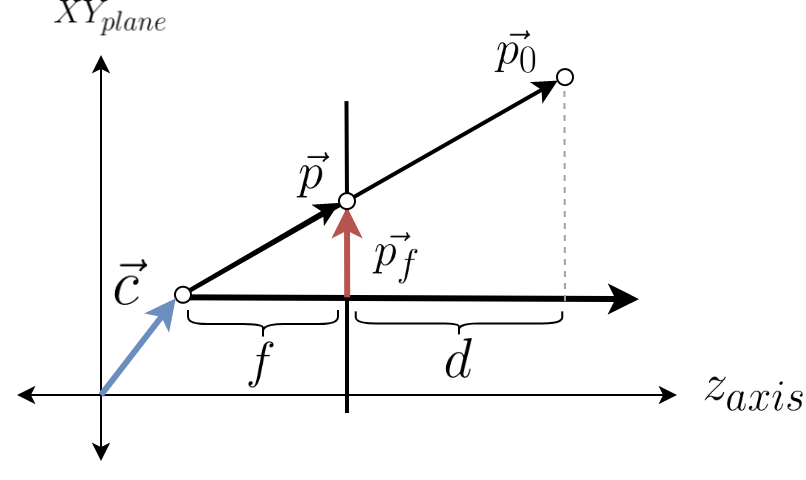
\includegraphics[width=8.5cm]{translated_3d.png}
\caption{3D projection with translated camera coordinates}
\label{fig:figure}
\end{figure} 
\noindent This issue can be resolved by simply applying a counter translation such that the camera moves back to the origin. The system can then be projected normally, just like in Section 4.1. Let the camera be represented by the position vector $\vec{c} = \begin{bmatrix}[0.5] c_x & c_y & c_z & 1\end{bmatrix}$, where $c_x, c_y, c_z \in \mathbb{R}$. Then, the counter translation matrix, $\mathbf{D_c}$, will be,
\begin{equation}
    \mathbf{D_c} = \begin{bmatrix}[0.5] 1 & 0 & 0 & 0 \\ 0 & 1 & 0 & 0 \\ 0 & 0 & 1 & 0 \\ -c_x & -c_y & -c_z & 1 \end{bmatrix}.
\end{equation}
Such that, $\vec{c}\;\mathbf{D_c} = \begin{bmatrix}[0.5](c_{x}-c_x)&(c_{y}-c_y)&(c_{z}-c_z)&1 \end{bmatrix} = \begin{bmatrix}[0.5]0&0&0&1 \end{bmatrix}$. (This is the homogeneous equivalent of the 0 vector and it is still the origin point)

\subsection{Rotated Camera Angle}
Just like how the camera coordinates can change, the angle of the camera can also change accordingly. The following diagram will outline the case where the normal vector of the projection plane does not lie on the z-axis.
\begin{figure}[H]
\centering
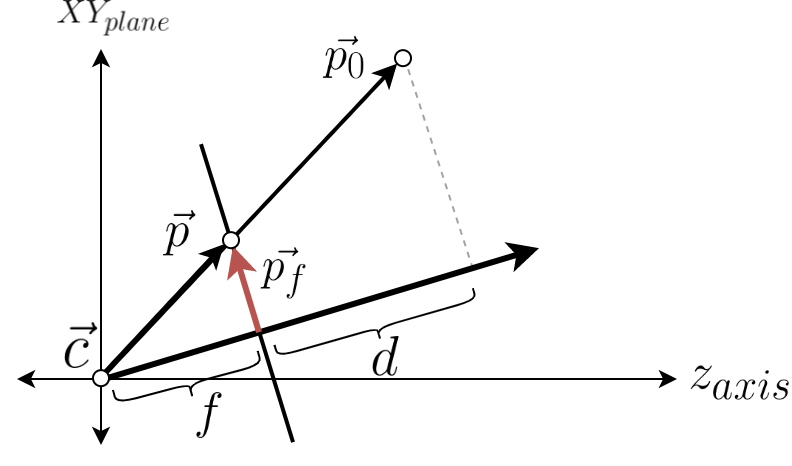
\includegraphics[width=8.5cm]{rotated_3d.png}
\caption{3D projection with rotated camera direction}
\label{fig:figure}
\end{figure} 
\noindent This system can be solved by counter-rotating, such that the axes of the camera system moves back onto the spacial axes. Although the direction of the camera can be directly determined by the normal vector of the projection plane, doing so will make camera angles unclear. Therefore, the direction is alternatively represented by a set of angles. As such, the goal state of the system will be where all the angles are 0. In 3D space, any direction vector can be determined with 3 angles $\alpha$, $\beta$, and $\gamma$, where $\alpha, \beta, \gamma \in \mathbb{R}$ (Figure 8).
\begin{figure}[H]
\centering
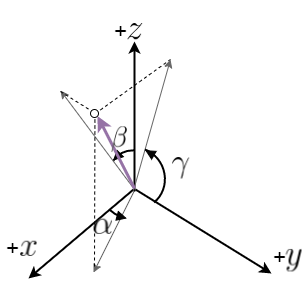
\includegraphics[width=6cm]{angles.png}
\caption{Diagram of how $\alpha$, $\beta$, and $\gamma$ are used to determine the direction in 3D space}
\label{fig:figure}
\end{figure} 
\noindent The change in each of those angles will coincide with a rotation about a different axis. As previously stated, a counter rotation will be done for each angle such that it returns to the simple case. These rotations will be done through a series of rotation matrices, $\mathbf{R_x}$, $\mathbf{R_y}$, and $\mathbf{R_z}$, each for a rotation about each axis. In order to form a generalized method used to derive the rotation matrices, it is important to understand the principles of how transformation matrices affect a vector. So, for a transformation matrix,

$\mathbf{T} = \begin{bmatrix}[0.5]\vec{r_1}&|&\vec{r_2}&|&\vec{r_3}&|&\vec{r_4}\end{bmatrix}^\intercal$ ($\vec{r_i} \in \mathbb{R}^4$ are the rows vectors of $\mathbf{T}$ because of the transpose),

\noindent applied on a 3D vector 
$$\vec{v} = \begin{bmatrix}[0.5]x&y&z&1\end{bmatrix} = x\vec{i} + y\vec{j} + z\vec{k} + 1\vec{l},$$
will result in a transformed vector, 
$$\vec{v} \; \mathbf{T} = x\vec{r_1} + y\vec{r_2} + z\vec{r_3} + 1\vec{r_4}.$$
The value of $\vec{r_4}$ should just be the original basis vector, $\vec{l}$, as the transformation should not effect the 1 at the end (it is only there to enable affine transformations). Upon closer inspection, this is the same effect as applying the transformation individually on each vector basis of the original space, where
\begin{equation}
    \vec{v} \; \mathbf{T} = x(\vec{i}\; \mathbf{T}) + y(\vec{j}\;\mathbf{T}) + z(\vec{k}\;\mathbf{T}) + 1\vec{l} = x\vec{r_1} + y\vec{r_2} + z\vec{r_3} + 1\vec{l}.
\end{equation}
Hence, to find the rotation matrix, the effects on each vector basis need to be individually calculated and joined together later. For example, the rotation matrix $\mathbf{R_z}$ will result in a rotation about the z-axis which affects the $x$ and $y$ values, or the $\vec{i}$ and the $\vec{j}$ basis. 
\begin{figure}[H]
\centering
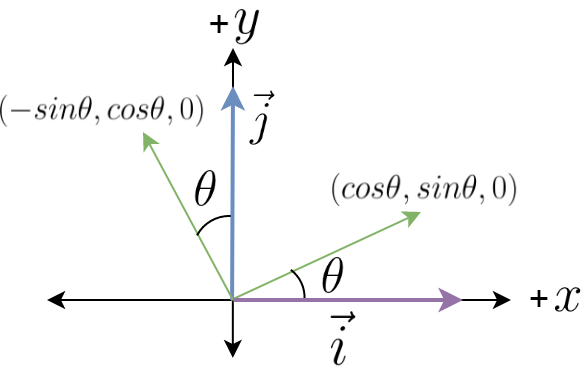
\includegraphics[width=8cm]{rotation_example.png}
\caption{Example of rotation about the z-axis (the z-axis is coming out of the page)}
\label{fig:figure}
\end{figure}
Using some simple trigonometry, the rotated coordinates of each basis can be calculated. Hence, for an angle $\theta \in \mathbb{R}$, the position vectors of the rotated $\vec{i}$ is $\begin{bmatrix}[0.5]cos\theta&sin\theta&0&0\end{bmatrix}$ and the rotated $\vec{j}$ is $\begin{bmatrix}[0.5]-sin\theta&cos\theta&0&0\end{bmatrix}$ (the new position vectors do not have homogeneous coordinates because the basis vectors do not have homogeneous coordinates either). The remaining vector bases, $\vec{k}$ and $\vec{l}$, are unchanged because the rotation does not influence them. Hence, the combined rotation matrix will be
$$\mathbf{R_z} = \begin{bmatrix}[0.5]cos\theta&sin\theta&0&0\\-sin\theta&cos\theta&0&0\\0&0&1&0\\0&0&0&1 \end{bmatrix}$$
Because the z-axis rotation is characterized by the angle $\alpha$, the counter rotation will have angles $-\alpha$. Therefore,
$$\mathbf{R_z} = \begin{bmatrix}[0.5]cos(-\alpha)&sin(-\alpha)&0&0\\-sin(-\alpha)&cos(-\alpha)&0&0\\0&0&1&0\\0&0&0&1 \end{bmatrix} = \begin{bmatrix}[0.5]cos(\alpha)&-sin(\alpha)&0&0\\sin(\alpha)&cos(\alpha)&0&0\\0&0&1&0\\0&0&0&1 \end{bmatrix}.$$

Using the same method for $R_x$ (affects $\vec{j}$ and $\vec{k}$), and $R_y$ (affects $\vec{i}$ and $\vec{k}$), will give
\begin{equation}
    \begin{gathered}
        \mathbf{R_x} = \begin{bmatrix}[0.5]1&0&0&0\\0&cos(\gamma)&-sin(\gamma)&0\\0&sin(\gamma)&cos(\gamma)&0\\0&0&0&1 \end{bmatrix}\;\;\mathbf{R_y} = \begin{bmatrix}[0.5]cos(\beta)&0&sin(\beta)&0\\0&1&0&0\\-sin(\beta)&0&cos(\beta)&0\\0&0&0&1 \end{bmatrix}\\ 
        \mathbf{R_z} = \begin{bmatrix}[0.5]cos(\alpha)&-sin(\alpha)&0&0\\sin(\alpha)&cos(\alpha)&0&0\\0&0&1&0\\0&0&0&1 \end{bmatrix}
    \end{gathered}
\end{equation}
\subsection{Combined Process}
The key of the combined process is to simplify the system such that it becomes the simple case. Therefore, the steps to this process will be
\begin{enumerate}
  \item Translate system such that the camera is at the origin (Section 4.2)
  \item Rotate system such that camera angles are all 0 (Section 4.3)
  \item Project the points (Section 4.1)
\end{enumerate}
This combination is achieved by multiplying all the different matrices together in that order (the ease of combination is also the reason why matrices were chosen).
\begin{equation*}
    \vec{p_f} = \vec{p_0} \mathbf{D_c}\mathbf{R_x}\mathbf{R_y}\mathbf{R_z}\mathbf{J},
\end{equation*}
where $\mathbf{D_c}$ is the translation matrix, $\mathbf{R_x}$, $\mathbf{R_y}$, and $\mathbf{R_z}$ are the rotation matrices, and $\mathbf{J}$ is the projection matrix. However, $\mathbf{J}$ will use values of the corrected vector, $\vec{p_0}\mathbf{D_c}\mathbf{R_x}\mathbf{R_y}\mathbf{R_z}$, as it needs the transformed coordinates of the original vector to calculate the final perspective scaling. Therefore, the actual projection matrix, $\mathbf{J}$, is rewritten as,
$$\mathbf{J_T} =\begin{bmatrix}[0.7] \frac{f}{p_{T, z}} & 0 & 0 & 0\\ 0 & \frac{f}{p_{T, z}} & 0 & 0 \\ 0 & 0 & \frac{f}{p_{T, z}} & 0 \\ 0 & 0 & -f & 1\\   \end{bmatrix},$$
where $\vec{p_T} = \vec{p_0}\mathbf{D_c}\mathbf{R_x}\mathbf{R_y}\mathbf{R_z}$. The final equation for 3D perspective projections will then be
\begin{equation}
    \vec{p_f} = \vec{p_0} \mathbf{D_c}\mathbf{R_x}\mathbf{R_y}\mathbf{R_z}\mathbf{J_T},
\end{equation}
where $\vec{p_f}, \vec{p_0} \in \mathbb{R}^4$. These matrices will not be condensed because it does not simplify the equation - it just makes it more convoluted and less intuitive. 

\section{4D Perspective Projections}
After establishing an understanding of 3D perspective projections, the IA can now move on to 4D perspective projections. Because it is impossible to visualize 4D space directly, a lot of the explanations will use analogies from lower dimensions. Moreover, the pre-established mathematical understanding from 3D projections can also be extended towards 4D projections. This section will discuss how to project 4D points onto 3D space, as points (vertices) are a key component of understanding 4D polygons.
\subsection{4D Projections}
 The entire perspective projection method will remain the same, with the exception that the depth, $d$, is now caused by the w-component (the 4th dimensional component). Hence, the translation at the end of the projection will be on the w-component of $\vec{p_0}$. This also holds true for any 4D position vector, $\vec{p_n} \in \mathbb{R}^5$, of a point. Hence, the general projection matrix for $\vec{p_n}$ is, 
\begin{equation}
    \mathbf{J_n} = \begin{bmatrix}[0.7] \frac{f}{p_{n, w}} & 0 & 0 & 0 & 0\\ 0 & \frac{f}{p_{n, w}} & 0 & 0 & 0 \\ 0 & 0 & \frac{f}{p_{n, w}} & 0 & 0 \\ 0 & 0 & 0 & \frac{f}{p_{n, w}} & 0  \\ 0 & 0 & 0 & -f & 1   \end{bmatrix}
\end{equation}
such that $\vec{p_f} = \vec{p_n}\mathbf{J_n}$ and $\vec{p_f}$ is the projected vector, where $\vec{p_f} \in \mathbb{R}^5$ while $f \in \mathbb{R}_{\geq0}$. When calculated correctly, $p_{f,w} = p_{n,w} \left( \frac{f}{p_{n,w}}\right) - f = 0$, which verifies that the final projected vector is in lower dimensional space.

\subsection{4D Translations}
Just like 3D translations, 4D translations allow the movement of the camera back to the origin. The only difference is the extra dimension. Hence, given a camera with a position vector of $\vec{c} = \begin{bmatrix}[0.5] c_x & c_y & c_z& c_w & 1\end{bmatrix}$ with $c_x, c_y, c_z, c_w \in \mathbb{R}$, the counter translation matrix will be,
\begin{equation}
    \mathbf{D_c} = \begin{bmatrix}[0.5] 1 & 0 & 0 & 0 & 0 \\ 0 & 1 & 0 & 0 & 0 \\ 0 & 0 & 1 & 0 & 0 \\ 0 & 0 & 0 & 1 & 0 \\ -c_x & -c_y & -c_z & -c_w & 1 \end{bmatrix}.
\end{equation}
\subsection{4D Rotations}
The process to solve for rotated camera angles in 4D is similar to that of 3D: find a counter-rotation matrix that can rotate the camera back into standard position. Although 4D rotations share similarities with 3D rotations, it still has distinct differences that need to be addressed. Because of their increased degree of freedom, 4D objects rotate through space differently than 3D. 4D objects rotate about planes, not lines. This concept is similar to how a 2D shape only rotates about a point. A rotation through a new spatial dimension also requires a spatial extension of the rotation center. To understand this better, rotations need to be visualized differently. Instead of thinking of rotations as movement around a stationary center, it is better to visualize rotations as a planar movement. To illustrate, a 2D rotation revolves around an object in a plane, but since there is only one 2D plane available in 2D space, the stationary center will be a point of 0 dimensions. Similarly, rotations in 3D also occur on a rotational plane, but since 3D has one extra dimension, the resulting stationary center will be a line. Lastly, rotations in 4D are also in a 2D rotational plane, so the resulting stationary center must be the leftover 2 dimensions, which is a plane. Because of this, there will be ${}_{4}C_{2} = 6$ different rotations in 4D space. To define these 6 rotations, 6 distinct angles, $\alpha$, $\beta$, $\gamma$, $\delta$, $\epsilon$, and $\zeta$ will be used, where $\alpha, \beta, \gamma, \delta, \epsilon, \zeta \in \mathbb{R}$. Each of these angles will pertain to a rotation matrix, $\mathbf{R_{xy}}$, $\mathbf{R_{yz}}$, $\mathbf{R_{xz}}$, $\mathbf{R_{xw}}$, $\mathbf{R_{yw}}$, and $\mathbf{R_{zw}}$. Since it is not possible to draw 4D axes, they will instead be broken down into three different 3D spatial axes. This works because all of the 4D axes are orthogonal to each other.
\begin{figure}[H]
\centering
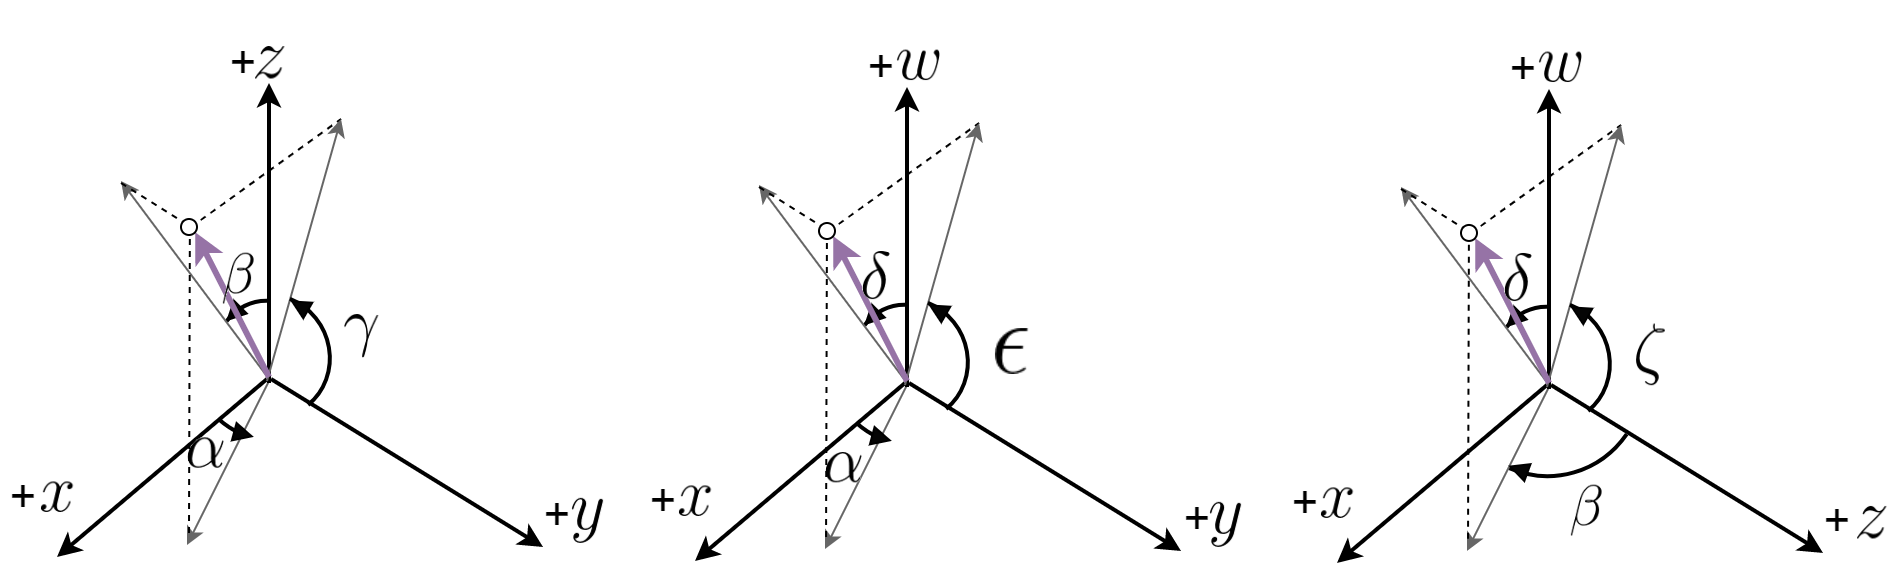
\includegraphics[width=17cm]{4d_angles.png}
\caption{Dissection of rotation angles for a 4D vector (diagram is not to scale nor geometrically accurate)}
\label{fig:figure}
\end{figure}
The derivation of the rotation matrices will remain the same as the 3D variation, where the transformation is just applied to the vector basis. But for 4D, there will be one extra vector basis and one additional dimension. For example, $\mathbf{R_{xy}}$ is the rotation about the $XY$ plane, which is a rotation in the $ZW$ plane.
\begin{figure}[H]
\centering
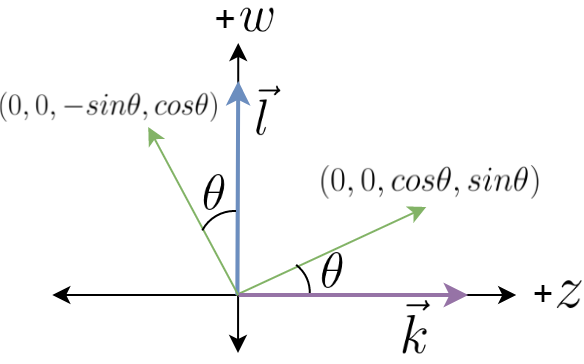
\includegraphics[width=7cm]{rotation_4d_example.png}
\caption{Example of 4D rotation about the XY plane}
\label{fig:figure}
\end{figure}
From the above diagram, for an angle $\theta \in \mathbb{R}$, the rotated value of $\vec{k}$ is $\begin{bmatrix}[0.5]0 & 0 & cos\theta & sin\theta & 0\end{bmatrix}$, and the rotated value of  $\vec{l}$  is $\begin{bmatrix}[0.5]0 & 0 & -sin\theta & cos\theta & 0\end{bmatrix}$. Moreover, since $\mathbf{R_{xy}}$ causes a rotation in the $ZW$ plane, the corresponding angle is $\zeta$, and the counter rotation angle will be $-\zeta$. Hence, combining all the transformed basis vectors will yield the counter rotation matrix, 
$$\mathbf{R_{xy}} = \begin{bmatrix}[0.5] 1 & 0 & 0 & 0 & 0 \\ 0 & 1 & 0 & 0 & 0\\ 0 & 0 & cos(-\zeta) & sin(-\zeta) & 0\\ 0 & 0 & -sin(-\zeta) & cos(-\zeta) & 0\\ 0 & 0 & 0 & 0 & 1\end{bmatrix} = \begin{bmatrix}[0.5] 1 & 0 & 0 & 0 & 0 \\ 0 & 1 & 0 & 0 & 0\\ 0 & 0 & cos(\zeta) & -sin(\zeta) & 0\\ 0 & 0 & sin(\zeta) & cos(\zeta) & 0\\ 0 & 0 & 0 & 0 & 1\end{bmatrix}.$$
Applying the same process for $\mathbf{R_{yz}}$ (Rotation on $XW$ plane; angle $\delta$), $\mathbf{R_{xz}}$ (Rotation on $YW$ plane; angle $\epsilon$), $\mathbf{R_{xw}}$ (Rotation on $YZ$ plane; angle $\gamma$), $\mathbf{R_{yw}}$ (Rotation on $XZ$ plane; angle $\beta$), and $\mathbf{R_{zw}}$ (Rotation on $XY$ plane; angle $\alpha$) gives the set of counter rotation matrices:

\begin{gather}
    \mathbf{R_{xy}} = \begin{bmatrix}[0.6] 1 & 0 & 0 & 0 & 0 \\ 0 & 1 & 0 & 0 & 0\\ 0 & 0 & cos(\zeta) & -sin(\zeta) & 0\\ 0 & 0 & sin(\zeta) & cos(\zeta) & 0\\ 0 & 0 & 0 & 0 & 1\end{bmatrix}\;\;
    \mathbf{R_{xz}} = \begin{bmatrix}[0.6] 1 & 0 & 0 & 0 & 0 \\ 0 & cos(\epsilon) & 0 & -sin(\epsilon) & 0\\ 0 & 0 & 1 & 0 & 0\\ 0 & sin(\epsilon) & 0 & cos(\epsilon) & 0\\ 0 & 0 & 0 & 0 & 1\end{bmatrix}\notag\\ 
    \mathbf{R_{yz}} = \begin{bmatrix}[0.6] cos(\delta) & 0 & 0 & sin(\delta) & 0 \\ 0 & 1 & 0 & 0 & 0\\ 0 & 0 & 1 & 0 & 0\\ -sin(\delta) & 0 & 0 & cos(\delta) & 0\\ 0 & 0 & 0 & 0 & 1\end{bmatrix}\;\;
    \mathbf{R_{xw}} = \begin{bmatrix}[0.6] 1 & 0 & 0 & 0 & 0 \\ 0 & cos(\gamma) & -sin(\gamma) & 0 & 0\\ 0 & sin(\gamma) & cos(\gamma) & 0 & 0\\ 0 & 0 & 0 & 1 & 0\\ 0 & 0 & 0 & 0 & 1\end{bmatrix}\\
    \mathbf{R_{yw}} = \begin{bmatrix}[0.6] cos(\beta) & 0 & sin(\beta) & 0 & 0 \\ 0 & 1 & 0 & 0 & 0\\ -sin(\beta) & 0 & cos(\beta) & 0 & 0\\ 0 & 0 & 0 & 1 & 0\\ 0 & 0 & 0 & 0 & 1\end{bmatrix}\;\;
    \mathbf{R_{zw}} = \begin{bmatrix}[0.6] cos(\alpha) & -sin(\alpha) & 0 & 0 & 0 \\ sin(\alpha) & cos(\alpha) & 0 & 0 & 0\\ 0 & 0 & 1 & 0 & 0\\ 0 & 0 & 0 & 1 & 0\\ 0 & 0 & 0 & 0 & 1\end{bmatrix}.\notag
\end{gather}


\subsection{Combined Projection Process}
The combined projection process in 4D will also move the system to the simple projection case. Therefore, the order of the process is the same as the 3D version:
\begin{enumerate}
  \item Translate system such that the camera is at the origin (Section 5.2)
  \item Rotate system such that camera angles are all 0 (Section 5.3)
  \item Project the points (Section 5.1)
\end{enumerate}
Given a camera with position vector $\vec{c} = \begin{bmatrix}[0.5] c_x & c_y & c_z& c_w & 1\end{bmatrix}$, defined by the angles $\alpha$, $\beta$, $\gamma$, $\delta$, $\epsilon$, and $\zeta$. The combined transformation on a 4D vector $\vec{p_0}$ gives the general equations:
\begin{equation}
    \begin{gathered}
\vec{p_T} = \vec{p_0} \mathbf{D_c}\mathbf{R_{xy}}\mathbf{R_{xz}}\mathbf{R_{yz}}\mathbf{R_{xw}}\mathbf{R_{yw}}\mathbf{R_{zw}}\\
\vec{p_f} = \vec{p_0} \mathbf{D_c}\mathbf{R_{xy}}\mathbf{R_{xz}}\mathbf{R_{yz}}\mathbf{R_{xw}}\mathbf{R_{yw}}\mathbf{R_{zw}}\mathbf{J_T} = \vec{p_T}\mathbf{J_T}.
    \end{gathered}
\end{equation}
Where $\vec{p_T} \in \mathbb{R}^5$ is the resultant from the matrix transformations, $\vec{p_f}$ is the resulting projection, $\mathbf{D_c}$ is the translation matrix, $\mathbf{R_{i}}$ are the 4D rotation matrices, and $\mathbf{J_T}$ is the projection matrix of $\vec{p_T}$. Note that the resulting vector, $\vec{p_f} \in \mathbb{R}^5$, should be in the form of $\begin{bmatrix}[0.5] p_{f,x} & p_{f,y} & p_{f,z} & 0 & 1\end{bmatrix}$. The w-component, $p_{f,w}$, is 0, which shows that the resulting projection is indeed in lower dimensional space. Therefore, the final vector with reduced dimensions ($\mathbb{R}^3$) for rendering is $\vec{p_f}' = \begin{bmatrix}[0.5] p_{f,x} & p_{f,y} & p_{f,z} \end{bmatrix}$ (homogeneous coordinates are removed, they are not required for rendering). To calculate this mathematically, $\vec{p_f}$ is multiplied by a $3 \times 5$ dimensional-reducing matrix, $\mathbf{P}$. Where
\begin{equation}
\mathbf{P} = \begin{bmatrix}[0.5] 1 & 0 & 0 \\ 0 & 1 & 0 \\ 0 & 0 & 1 \\0 & 0 & 0 \\ 0 & 0 & 0\end{bmatrix} \text{ and }
    \vec{p_f}' = \vec{p_0} \mathbf{D_c}\mathbf{R_{xy}}\mathbf{R_{xz}}\mathbf{R_{yz}}\mathbf{R_{xw}}\mathbf{R_{yw}}\mathbf{R_{zw}}\mathbf{J_T}\mathbf{P} = \vec{p_T}\mathbf{J_T}\mathbf{P}.
\end{equation}
\subsubsection{Dealing With Edges}
 Edges are a crucial part of visualizing polygons. An edge is defined as a line connecting a pair of points. Because an edge is a line with no thickness, its projection process is relatively simple. Instead of dealing with additional calculations, the projected edge in 3D can be reconstructed with the two known projected vertices. The relationship of an edge will remain the same despite projection; the edge connecting $p_1$ and $p_2$ will also be true after projection. Hence, a simple line is just drawn between the two corresponding projected points. 

\section{Programmatic Implementation}
 To verify the results, the general equation is implemented programmatically in JavaScript. The following algorithm will outline the general process.
\begin{algorithm}[H]
\caption{4D Perspective Projection Implementation}
\begin{algorithmic}[1]
\STATE $\mathbf{D_c} = computeTranslationMatrix()$
\STATE $\mathbf{R_{xy}},\; \mathbf{R_{xz}},\; \mathbf{R_{yz}},\; \mathbf{R_{xw}},\; \mathbf{R_{yw}},\; \mathbf{R_{zw}} \leftarrow computeRotationMatrices()$

\FORALL{$p_{i} \in \mathbb{R}^4$}
    \STATE $\vec{p_T} = \vec{p_0}\mathbf{D_c}\mathbf{R_{xy}}\mathbf{R_{xz}}\mathbf{R_{yz}}\mathbf{R_{xw}}\mathbf{R_{yw}}\mathbf{R_{zw}}$
    \STATE $\mathbf{J_T} \leftarrow computeProjectionMatrix(\vec{p_T})$
    \STATE $\vec{p_f} = \vec{p_T} \mathbf{J_T}$
    \STATE $Draw\; \vec{p_f}$
\ENDFOR
\FORALL{$edge_{i} \in \mathbb{R}^4$}
    \STATE // an edge is simply a relationship between 2 points, this relationship is retained during projections 
    \STATE $Draw\; edge_{i}$
\ENDFOR
\end{algorithmic}
\end{algorithm}
\noindent A 4D object in the implementation will consist of a set of 4D points and a set of edges that connect certain points together. To aid the evaluation, a popular 4D shape, the tesseract, is used during the 4D perspective projection process. A tesseract is the 4D equivalent of a cube, and for this particular implementation, it will have a side length of 200 and the center at the origin. The position the 4D camera will be defined using homogeneous coordinates as $\vec{c} = \begin{bmatrix}[0.5] 0 & 0 & 0& -90 & 1\end{bmatrix}$. The focal distance, $f$, will be 100. Additionally, the angles $\alpha$, $\beta$, $\gamma$, $\delta$, $\epsilon$, and $\zeta$ are all initially 0. In the 3D view, the center of the page is the origin, while the left-right direction corresponds to the x-coordinates, the up-down direction to the y-coordinates, and the depth to the z-coordinates. Access to the implementation is available in the Appendix.

\section{Evaluation and Reflection}
The initially loaded projection of the tesseract is given below. The results are similar to projections outlined in Helmenstine's article.
\begin{figure}[H]
\centering
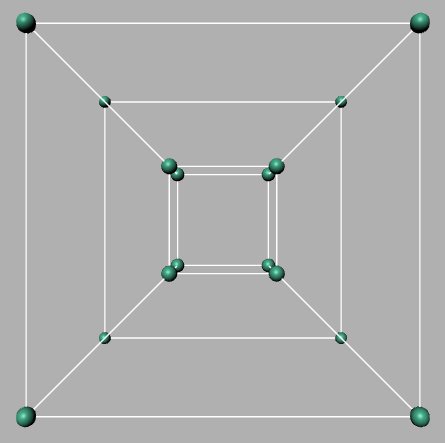
\includegraphics[width=4.5cm]{initial_tesseract.png}
\caption{Initial perspective projection of the tesseract}
\label{fig:figure}
\end{figure}

Next, the initial parameters will be altered to evaluate how the projection behaves. First, the angle parameters will be altered. Each angle corresponds to a rotation of the camera direction, and it yields different projections. From experimentation, camera rotations can be generalized into 2 categories: rotations that do not affect the w-component ($\mathbf{R_{xw}}$, $\mathbf{R_{yw}}$, $\mathbf{R_{zw}}$) and rotations that do affect the w-component ($\mathbf{R_{xy}}$, $\mathbf{R_{yz}}$, $\mathbf{R_{xz}}$). Rotations that do not affect the w-component exhibit clear rotation behaviour: 
\begin{figure}[H]
\centering
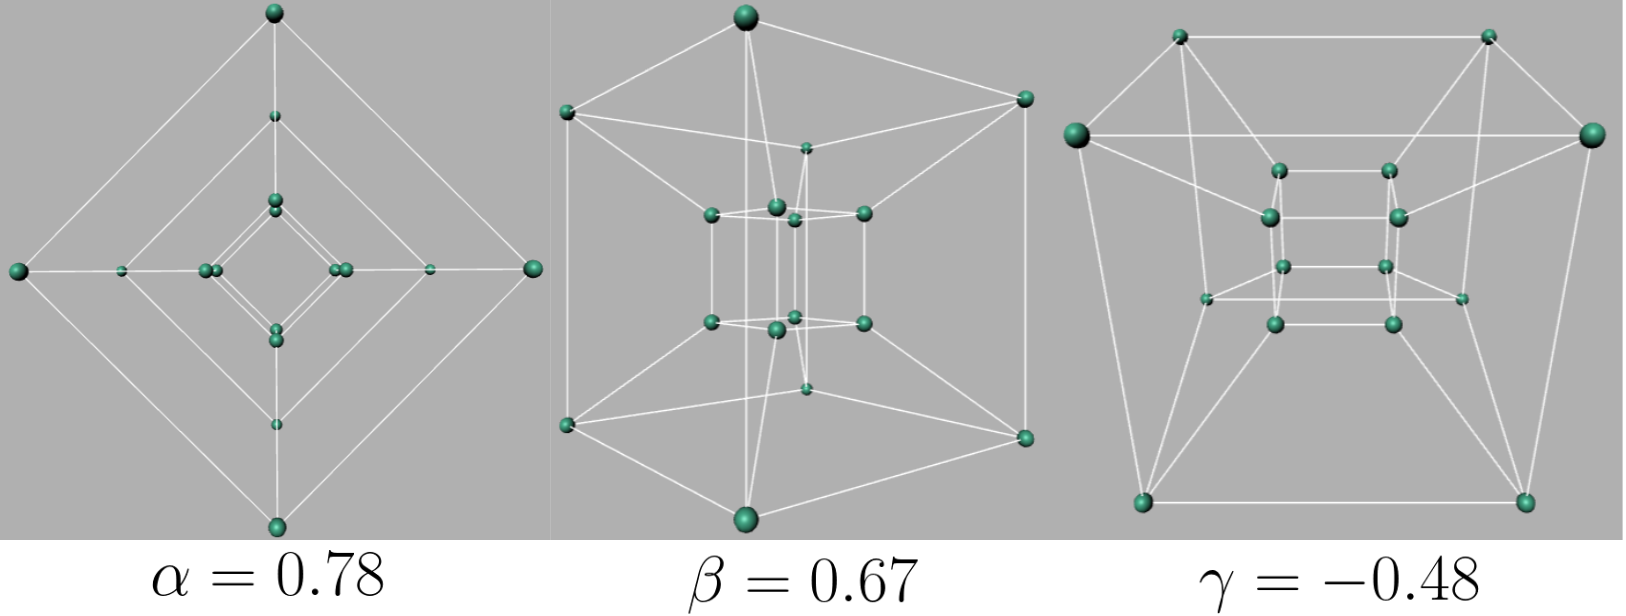
\includegraphics[width=13cm]{4D_rotation_no_W.png}
\caption{Projection as a result of $\mathbf{R_{xw}}$, $\mathbf{R_{yw}}$, $\mathbf{R_{zw}}$ (angles are in radians)}
\label{fig:figure}
\end{figure}
Upon closer inspection, the results are identical to directly rotating the 3D projection. Intuitively, this makes sense because each of those angles corresponds to a rotation about a 2D plane that exists in 3D space. For example, $\mathbf{R_{zw}}$ results in a rotation in the $XY$ plane, characterized by the angle $\alpha$. Moreover, because the perspective from the 4D projection is caused by the $w$ component, $\mathbf{R_{zw}}$ will not affect the perspective of the final project. Therefore, changing $\alpha$ will simply cause a rotation in the $XY$ plane about the z-axis for the 3D projection. To put mathematically, 
$$\vec{p_0}\mathbf{R_{nw}} = \vec{p_f}\mathbf{R_{n}},$$
where $n$ is the axis for the $NW$ plane that $\mathbf{R_{nw}}$ revolves around, and $\mathbf{R_{n}}$ is the 3D rotation matrix that describes a rotation about the n-axis.

However, rotations that affect the w-component are much more complex and cause the projection to warp. Just to reiterate, all rotations discussed in this section pertain to the rotation of the camera direction, not of the objects themselves. Rotations that affect the w-component seem to skew the projection:
\begin{figure}[H]
\centering
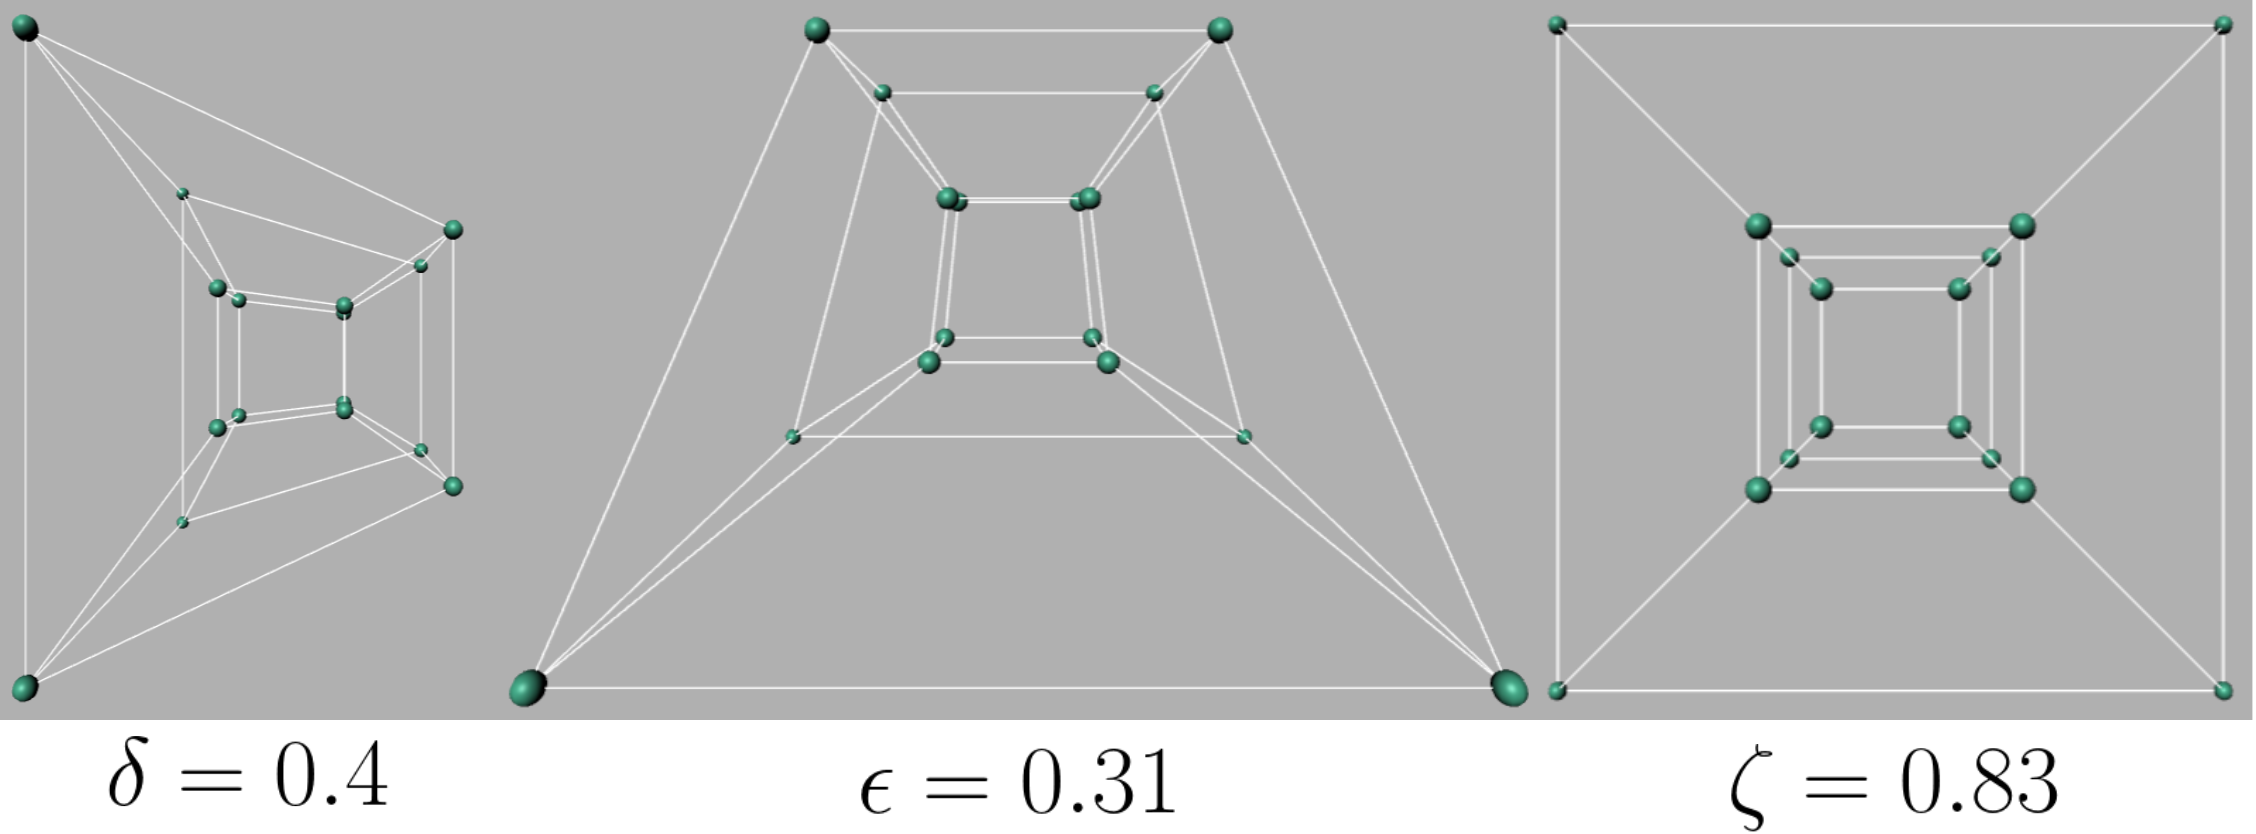
\includegraphics[width=14cm]{rotation+with_w.png}
\caption{Projection as a result of $\mathbf{R_{xy}}$, $\mathbf{R_{yz}}$, $\mathbf{R_{xz}}$ (angles are in radians)}
\label{fig:figure}
\end{figure}
The skew and scaling effects imply the existence of angle boundaries or else the scaling will be infinite. The maximum angle depends on the position of $\vec{p_0}$ and will occur when the rotation causes the 3D projection space to intersect with $\vec{p_0}$ in 4D. Turning any further from this angle will cause the camera view to exclude the 4D space of the object in it. To help visualize this explanation, a 3D case is drawn below:
\begin{figure}[H]
\centering
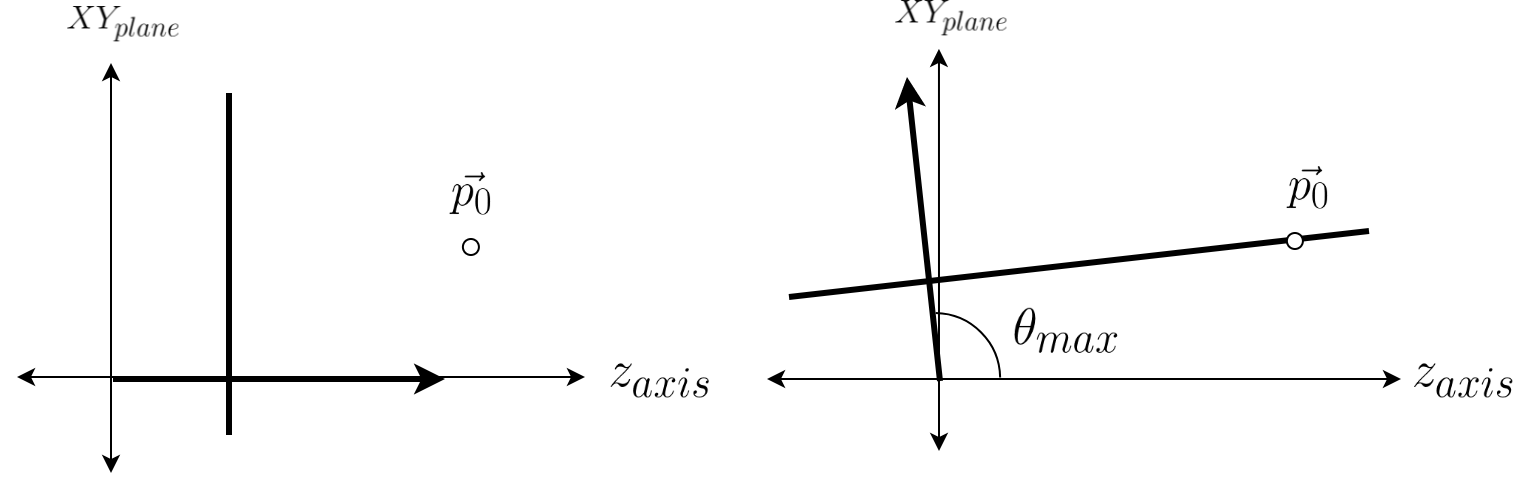
\includegraphics[width=12cm]{max_rotation.png}
\caption{Diagram of the maximum rotation angle ($\theta_{max}$) for a point $p_0$}
\label{fig:figure}
\end{figure}

Moving on, each of the camera coordinates, $c_x$, $c_y$, $c_z$, and $c_w$, will be modified. The last coordinate, $w$ is a special case as it directly affects the 4D depth and the sense of perspective of the 3D projection. The rest of the coordinates only shift and scale the projection.
\begin{figure}[H]
\centering
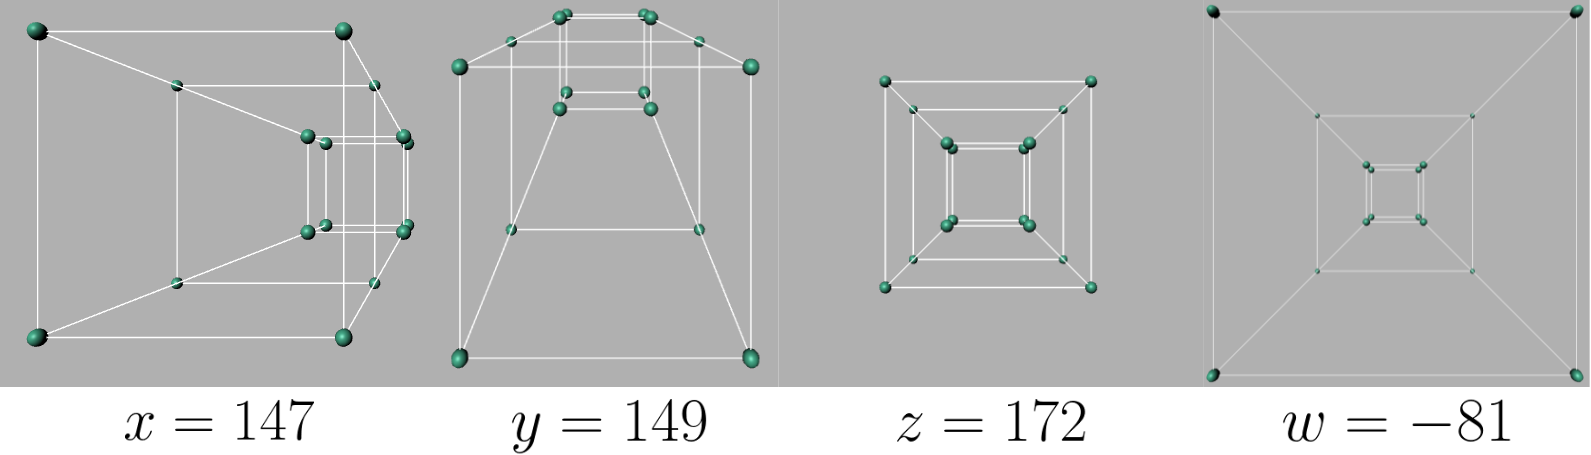
\includegraphics[width=17cm]{camera_coordinates.png}
\caption{Resulting projection from changing camera coordinates x, y, z, and w (originally $x,y,z = 0$ and $w = -90$)}
\label{fig:figure}
\end{figure}
Changing $c_x$, $c_y$, and $c_z$, causes a linear translation and scaling along that axis. This can be demonstrated using the derived 4D projection method. Assuming no other rotations, Equation 10 becomes, 
$$\vec{p_f} = \vec{p_0}\mathbf{D_c}\mathbf{J} = \vec{p_0}\begin{bmatrix}[0.5] 1 & 0 & 0 & 0 & 0 \\ 0 & 1 & 0 & 0 & 0 \\ 0 & 0 & 1 & 0 & 0 \\ 0 & 0 & 0 & 1 & 0 \\ -c_x & -c_y & -c_z & -c_w & 1 \end{bmatrix} \begin{bmatrix}[0.6] \frac{f}{p_{T, w}} & 0 & 0 & 0 & 0\\ 0 & \frac{f}{p_{T, w}} & 0 & 0 & 0 \\ 0 & 0 & \frac{f}{p_{T, w}} & 0 & 0 \\ 0 & 0 & 0 & \frac{f}{p_{T, w}} & 0  \\ 0 & 0 & 0 & -f & 1   \end{bmatrix}$$
$$=\vec{p_0} \begin{bmatrix}[0.6] \frac{f}{p_{T, w}} & 0 & 0 & 0 & 0\\ 0 & \frac{f}{p_{T, w}} & 0 & 0 & 0 \\ 0 & 0 & \frac{f}{p_{T, w}} & 0 & 0 \\ 0 & 0 & 0 & \frac{f}{p_{T, w}} & 0  \\ -c_x\frac{f}{p_{T, w}} & -c_y\frac{f}{p_{T, w}} & -c_z\frac{f}{p_{T, w}} & -f-c_w\frac{f}{p_{T, w}} & 1   \end{bmatrix}.$$
It is evident from the derived matrix that a change in either $c_n,\;n \in x,y,z$, will result in $p_{f, n} = \frac{f}{p_{T, w}}(p_{0,n}-c_n)$ (a translation then scaling) where $\vec{p_T} = \vec{p_0}\mathbf{D_c}$. However, a change in $c_w$ differs because it will directly change the value of $\frac{f}{p_{T,w}}$, therefore affecting the degree of scaling for all the projected vectors. Moreover, $p_{f,w} = \frac{f}{p_{T, w}}(p_{0,n} - c_n) - f = f-f = 0$, unlike the  other terms. Larger $|c_n|$ results in a smaller image, just like how 3D objects look smaller when they are further away.

This leads to the next and last parameter, the focal length $f$. This parameter, along with $c_w$, is responsible for the amount of perspective in the projection. 
\begin{figure}[H]
\centering
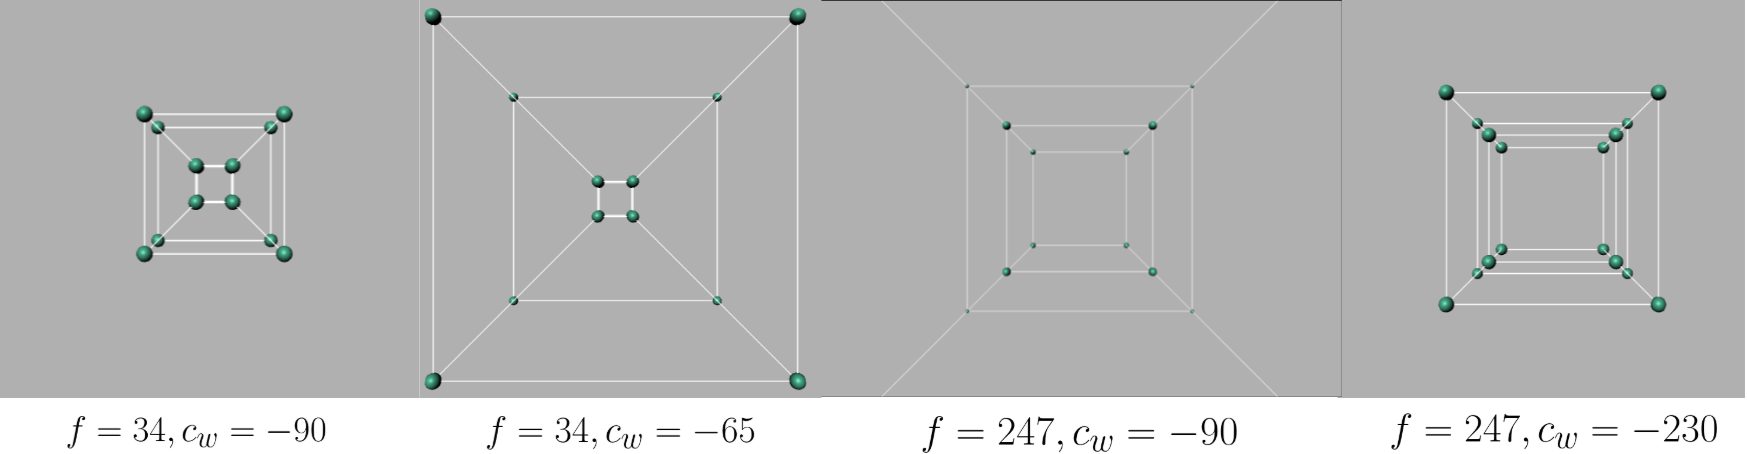
\includegraphics[width=17cm]{f_diagram.png}
\caption{Change of perspective resulting from changing $f$ values}
\label{fig:figure}
\end{figure}
The $c_w$ in the above figure only serves to zoom in to or out of the projected image. Decreasing the focal distance, $f$, changes the perspective by making the perspective effect more pronounced. In other words, closer points are scaled much larger, and further points are scaled smaller. Conversely, increasing $f$ causes the perspective effect to decrease, and points will be scaled less regardless of their distance from the camera. This perspective scaling directly corresponds to the ratio $\frac{f}{p_{T,w}}$. In a way, rather than being a literal focal distance, $f$ becomes more of a abstract scaling parameter that changes the degree of perspective. Interestingly, $\lim_{f\to\infty}\frac{f}{p_{T,w}} = \infty$, which seemingly does not result in useful projection results. Understanding this limit requires taking a look at Figure 5. When $f$ is approaching infinity, the perspective triangle will not exist, and there will only be a set of parallel lines. Hence, any projections in this form will not show any perspective, and they are called orthogonal projections (projection is achieved by directly displacing $\vec{p_0}$ by a vector orthogonal to the projected space). On the other hand, when $f$ approaches 0, $\lim_{f\to 0}\frac{f}{p_{T,w}} = 0$, and all projections decompose into the origin. 

\subsection{Limitations and Extensions}
 Firstly, planes are not considered in the projection, and this results in a confusing wireframe model that cannot fully demonstrate what a 4D polygon looks like. Perhaps an extension similar to the edge treatment (Subsection 5.4.1) could be added to render planes. Moreover, lighting in 4D is also not taken into consideration. This is partially because objects are a wireframe model, where no lighting can be considered at all. This is a significant limitation as lighting is an important part of computer graphics, and it can also help enhance the comprehensibility of the projected result. Hence, lighting is also a recommended addition in the future. 

Viewport clipping is also not considered in this IA. In real life, the size of the projected space is constrained, just like how a human retina has a set size. Instead, the method in this IA assumes an infinitely large projected space with no angle constraints. Sometimes, the implementation encounters erroneous rendering in viewing dead zones. A 4D viewing dead zone is analogously represented in 3D below. 
\begin{figure}[H]
\centering
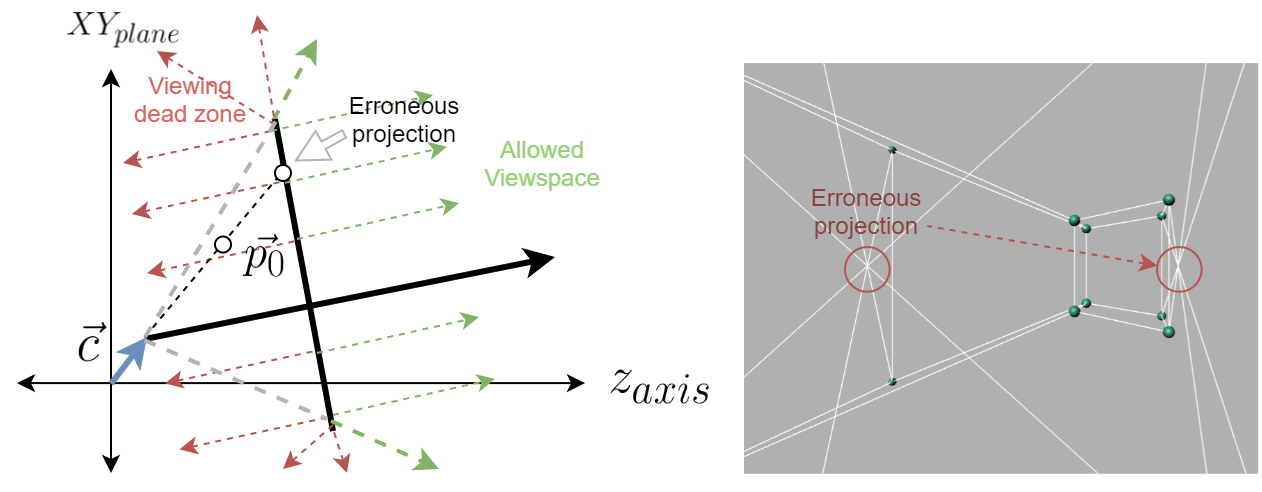
\includegraphics[width=15cm]{deadzone.png}
\caption{Erroneous rendering of $p_0$ in visual dead zones (Left: 3D explanation. Right: observed 4D example)}
\label{fig:figure}
\end{figure}
The addition of a viewport clipping algorithm should be considered for the future. Furthermore, FOV (Field of View) is an important concept that this IA does not consider explicitly. FOV provides a more realistic projection method as it is closely related to sight and perspective. Extensions regarding the use of FOV angles in the final projection equation are a recommended addition. Lastly, the set of matrices required for perspective projection is quite resource-intensive. Namely, the trigonometric functions in the rotation matrices are expensive to compute. Perhaps a better and more efficient method is available that can avoid the tedious rotation matrices.

\section{Conclusion}
 For this IA, a generalized method was developed to render 4D polygons that only consist of vertices and edges. The final method is mathematically written as a matrix transformation (Equation 11), that takes into account translated and rotated cameras. Additionally, this method was implemented with JavaScript to evaluate its efficacy (Section 6). Overall, the method behaves as expected and was able to render a tesseract with variable camera parameters. However, the current system has flaws such as the lack of lighting, planar rendering, viewport clipping, and explicit FOV consideration. 

Although 4D rendering may seem vague and not obviously useful, it can actually be used in some fields of physics. For example, the crystal structure of quasi-crystals in material science is studied with the help of 4D projections onto 3D space (Shahani). Perhaps the predominant use of 4D rendering would be its use in understanding space-time. The transformations developed in this IA can be applied to tangible scientific theories, one of them being Lorentz transformations. Moreover, investigating higher dimensions is very mathematically beautiful, and it can enhance the understanding of human observable spatial dimensions. Sometimes, it is worth it to do math just for the sake of doing math, and for the inherent satisfaction and beauty the process brings. I felt that this process has been very helpful in my journey in computer graphics; the mathematics learned is undoubtedly extremely useful for higher-level investigations. Similarly, the development of a basic 4D rendering engine opened plenty of intriguing and artistic paths of investigation for the future. 
\clearpage

\section{Bibliography}
\noindent
\vspace{-2em}
\setlength{\parindent}{-0.5in}
\setlength{\leftskip}{0.5in}
%\setlength{\parskip}{15pt}

Helmenstine, Anne. “What Is a Tesseract or Hypercube?” Science Notes and Projects, 19 Dec. 2021, sciencenotes.org/tesseract/.  Accessed Jan 1, 2022.

Shahani, Ashwin J, et al. “Now Showing in 4D: Quasicrystal Growth and Dissolution.” Aperiodic 2018 ("9th Conference on Aperiodic Crystals"), 2018, doi:10.31274/aperiodic2018-180810-51. 

Strang, Gilbert. Introduction to Linear Algebra. Wellesley-Cambridge Press, 2003.

\vspace{1em}
\setlength{\parindent}{0.5in}
\setlength{\leftskip}{0cm}

\section{Appendix}

The implementation demonstration is a website that requires WebGL and javaScript. It will most likely work on any modern browser on a computer.

\noindent Implementation: \url{https://onlinedocumentation.github.io/4dprojection/}

\noindent Source Code: \url{https://github.com/onlineDocumentation/4dprojection}

\end{document}
